\section{Cross-linking research data}

\begin{frame}{Cross-linking data, source code and reports/publications} 
	\framesubtitle{Schematic diagram}
	
	\begin{center}
		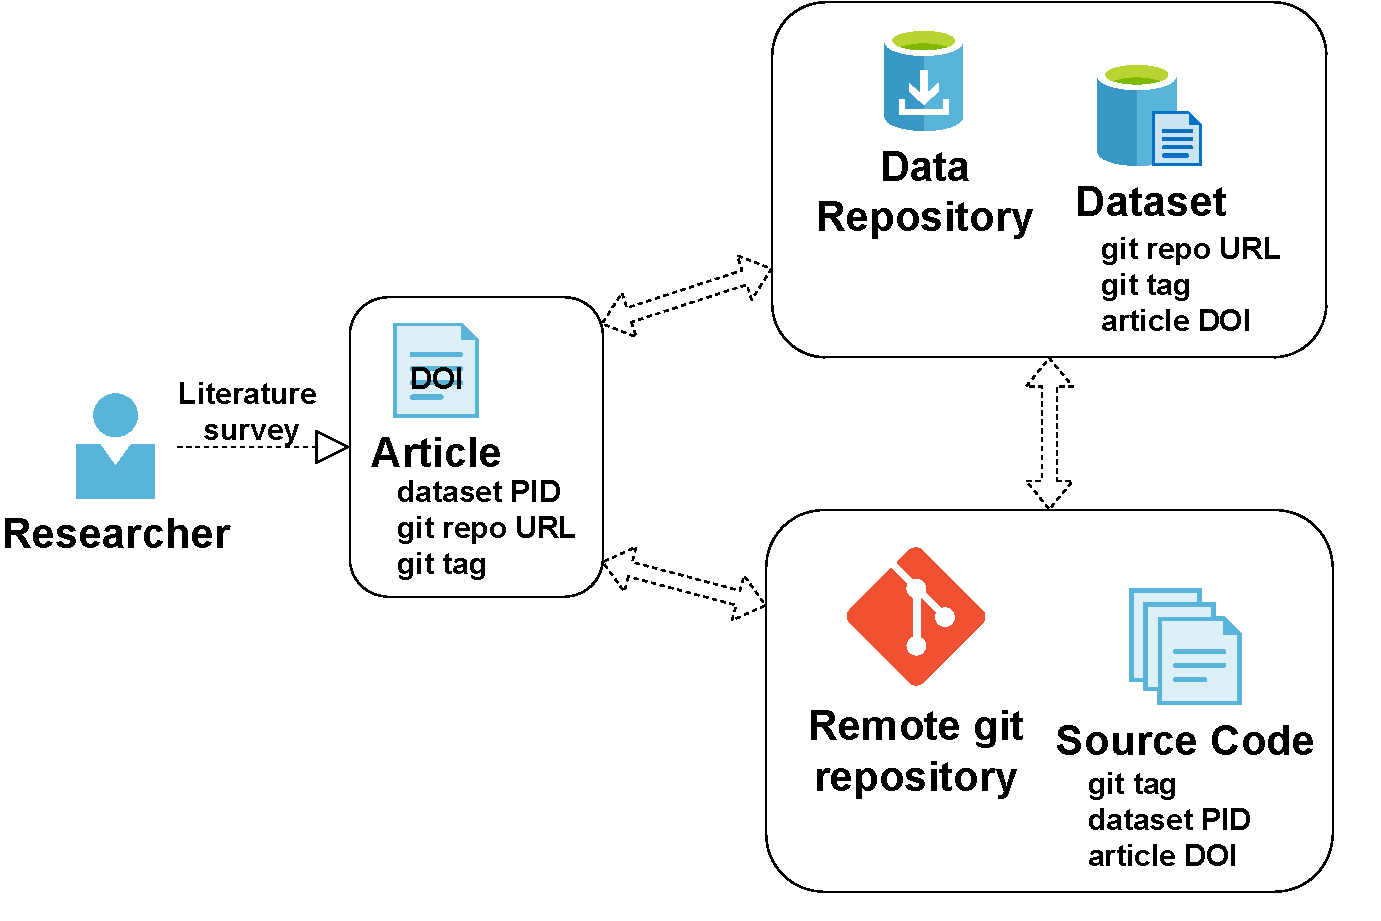
\includegraphics[width=0.67\textwidth]{figures/cross-linking.pdf}
	\end{center}

\end{frame}

\begin{frame}{(Cross-linking data, source code and reports/publications)} 
    \framesubtitle{Singularity} 
        
    \vfill
    \begin{itemize}
        \item Whence the Singularity Image\footnote{https://sylabs.io/docs/}?
            \begin{itemize}
                \item More intuitive than Docker: \textbf{Singularity handles images as files.} 
                \item Built for HPC from the start. 
                \item Doesn't require root rights. 
                \item Results as \emph{actual files}, not "data in spinning containers". 
                \item Maps user folder to the container: result data remains on the host. 
            \end{itemize}
        \item Why not replace Docker with Singularity within GitLab CI? 
            \begin{itemize}
                \item We're learning how to do this using \href{https://docs.gitlab.com/runner/executors/custom.html}{GitLab custom executors}.
                \item Does the workflow still survive publish-or-perish \faGraduationCap test?
            \end{itemize}
        \item Why a source-code snapshot on-top of the image and the repository? 
            \begin{itemize}
                \item Repositories get migrated, deleted, and some researchers still fear images. 
                \item Quick and direct access to source code from the publication. 
            \end{itemize}
    \end{itemize}

\end{frame}

\begin{frame}{(Cross-linking data, source code and reports/publications)} 
    \framesubtitle{Singularity simplifies reproducibility}

    \begin{itemize}
        \item The source code and the data stored in the image can be quickly reproduced.
        \item Article reviewers can clone, build, run and visualize easily. 
    \end{itemize}

    \href{https://git.rwth-aachen.de/leia/geophase/-/blob/JCOMP-D-19-01329R2/geophase.def}{Example: Singularity Image from an active review}
    \begin{itemize}
        \item Clone the code repository from the image: \\ \texttt{geophase-JCOMP-D-19-01329R2.sif clone geophase}
        \item Build: \\ \texttt{geophase-JCOMP-D-19-01329R2.sif build geophase build}
        \item Run tests: \\ \texttt{geophase-JCOMP-D-19-01329R2.sif run-tests geophase build}
        \item Open the jupyter notebook: \\ \texttt{geophase-JCOMP-D-19-01329R2.sif jupyter-notebook geophase}
    \end{itemize}

\end{frame}
